% !TeX spellcheck = <none>
% !TeX encoding = UTF-8
% !TeX root = main.tex

\chapter{LiDAR数据处理} % Chapter LiDAR数据处理

\section{点云滤波} 
\subsection{点云滤波概述}

\paragraph{点云滤波的目的}
\begin{itemize}
	\item LiDAR点云包括:地面点、 房屋点、树木、交通工具……。通过点云滤波来提取地面点,剔除非地面点。
	\item 基于LiDAR点云生成DEM:从点云中识别出地面点,并剔除建筑物、树木等非地面点,接着利用地面点生成DEM。
\end{itemize}

\paragraph{基于LiDAR数据生成DEM的工作}
\begin{itemize}
	\item 点云滤波
	\item DEM内插
	\item DEM精度分析
\end{itemize}

\paragraph{点云(距离数据)空间分布特征}
\begin{itemize}
	\item 地形平坦区域,由于激光脉冲的发射频率一般是固定的,激光点云在空间上成规则分布;
	\item 植被覆盖区域,点云之间的规则间隔被打破,由于脉冲可以穿透植被形成多次回波,空间分布成团聚等不规则形状;
	\item 水、云、雨或烟雾等能吸收近红外波段的激光脉冲,造成局部区域的点云缺失;
	\item 玻璃、光亮金属或建筑物边缘等表面的强反射,以及脉冲的折射、多路效应等,会引起点云的$ x $、$ y $或$ z $值异常,产生噪点。
\end{itemize}
一般情况下:
\begin{itemize}
	\item 建筑物和高大植被点云都具有较大的$ z $值(在城区,最大$ z $值的点云一般都是建筑物);
	\item 裸露地表点云的$ z $值最小;
	\item \textit{地面突出物}(如围墙、立交桥、花坛等)和灌丛点云的$ z $值介于两者之间;
\end{itemize}
这些地物在垂直方向上形成层次分布,而在
相邻地物之间,由于地面与地物的高度差异明显,
往往表现出高程突变现象,这就为地面点的识别
提供了依据。

\paragraph{基于高程突变的的滤波方法基本前提}
\begin{itemize}
	\item DSM中非地面点高于地面点(DEM)
	\item 地面点高程变化不会太大
\end{itemize}

\paragraph{自动滤波算法的难点}
\begin{enumerate}
	\item 局外点的影响,如图\ref{fig:局外点的影响}所示。
		\begin{figure}[htbp]
			\centering
			\quad\quad
			\subfloat[高的局外点]{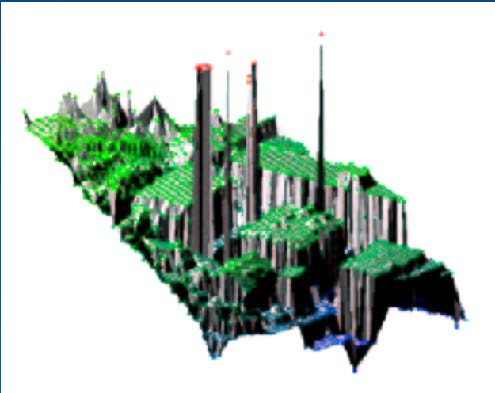
\includegraphics[height=3.5cm]{figure/Chapter6/高的局外点}} \hfill
			\subfloat[低的局外点]{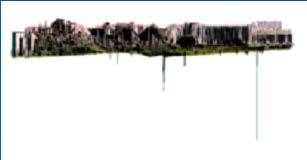
\includegraphics[height=3.5cm]{figure/Chapter6/低的局外点}} \hfill
			\subfloat[低的局外点导致侵蚀]{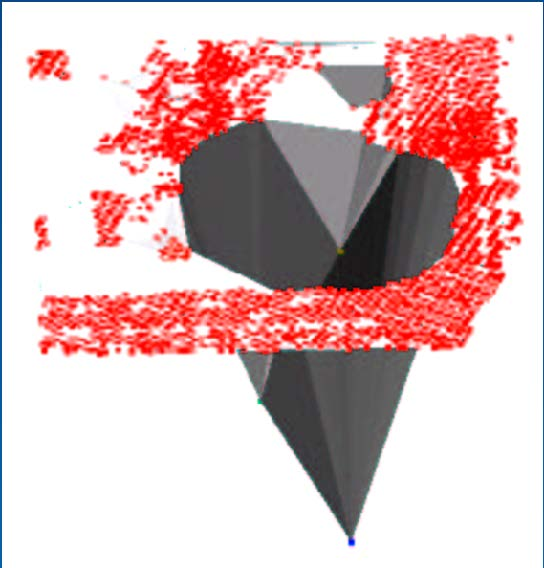
\includegraphics[height=3.5cm]{figure/Chapter6/低的局外点导致侵蚀}} \quad\quad
			\caption{局外点的影响}
			\label{fig:局外点的影响}
		\end{figure}
	\item 对象的复杂性、附着对象、点云分布不均匀、有断裂。
\end{enumerate}

\paragraph{滤波精度分析方法}
\begin{enumerate}
	\item \textit{第一类错误率}(Type I):将地面点分为地物点。
	\item \textit{第二类错误率}(Type II):将地物点分为地面点。
	\item \textit{总错误率}
\end{enumerate}

\paragraph{LiDAR点云滤波研究现状}如表\ref{tab:LiDAR点云滤波研究现状}所示。
\begin{table}[htbp]
	\centering
	\caption{LiDAR点云滤波研究现状}
	\label{tab:LiDAR点云滤波研究现状}
	\begin{tabular}{|l|l|}
		\hline
		假设条件         & 存在问题                        \\ \hline
		非地面点均高于地面点   & 由于粗差、多路径效应等,造成最低点并非理想地面点数据。 \\ \hline
		激光点可穿透树林到达地面 & 植被非常密集的地区,激光点难以穿过树林。        \\ \hline
		地形坡度不会过大     & 在平坦地区此假设有效,对坡度大的山区,并不总是满足   \\ \hline
	\end{tabular}
\end{table}

\paragraph{滤波算法研究趋势}
\begin{itemize}
	\item 高精度
	\item 全自动
	\item 高性能运算
	\item 融合辅助数据源的滤波优化算法
\end{itemize}

\subsection{典型滤波方法}

\kaiparagraph{一维双向扫描标记法}
\begin{enumerate}
	\item \textbf{算法思想}
		\begin{itemize}
			\item 认为非地面点与地面点构成的坡度大于地面点之间构成的坡度;
			\item 认为地面点的高程,低于邻域非地面点的高程。
		\end{itemize}
	\item \textbf{地面店判别条件}:
		\begin{equation}
		\forall P_i : \left\lbrace \begin{array}{ll}
		S_v > S_T ∧ Z_i > Z_T, & \text{地面点} \\
		\text{else},			& \text{非地面点}
		\end{array} \right.
		\end{equation}
	\item \textbf{算法步骤}
		\begin{enumerate}
			\item \textbf{基于高程和坡度条件扫描标记出初始地面点}:假设起始点为房屋点,根据坡度与高程阈值按从右到左、从左到右进行识别标记
				\begin{equation}
				S_i = \arctan \left[ \dfrac{Z_i - Z_{i-1}}{\sqrt{\left(X_i - X_{i-1}\right)^2 + \left(Y_i - Y_{i-1}\right)^2}} \right],\quad S_i \in \left[-\dfrac{\cpi}{2}, \dfrac{\cpi}{2}\right]
				\end{equation}
			\item \textbf{基于线性衰退法进一步去除非地面点}:认为局部区域地面点构成坡度一致,利用线性衰减法进一步去除非地面点
				\begin{equation}
				Z = a_0 + a_1D, \quad D < D_T
				\end{equation}
		\end{enumerate}
	\item \textbf{实例}:如图\ref{fig:一维双向扫描标记法算法步骤}所示。
		\begin{figure}[htbp]
			\centering
			\subfloat[原始点云]{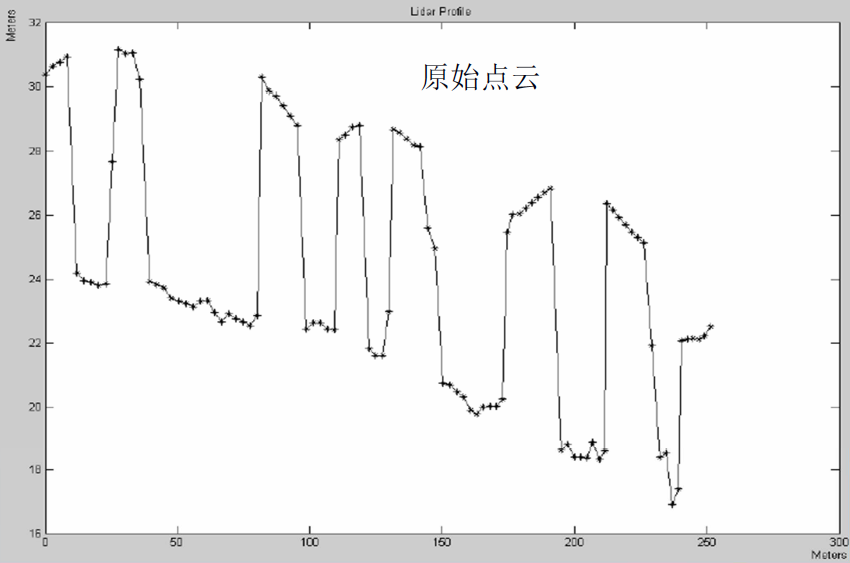
\includegraphics[height=3cm]{figure/Chapter6/一维双向扫描标记法-原始点云}} \quad
			\subfloat[从右往左]{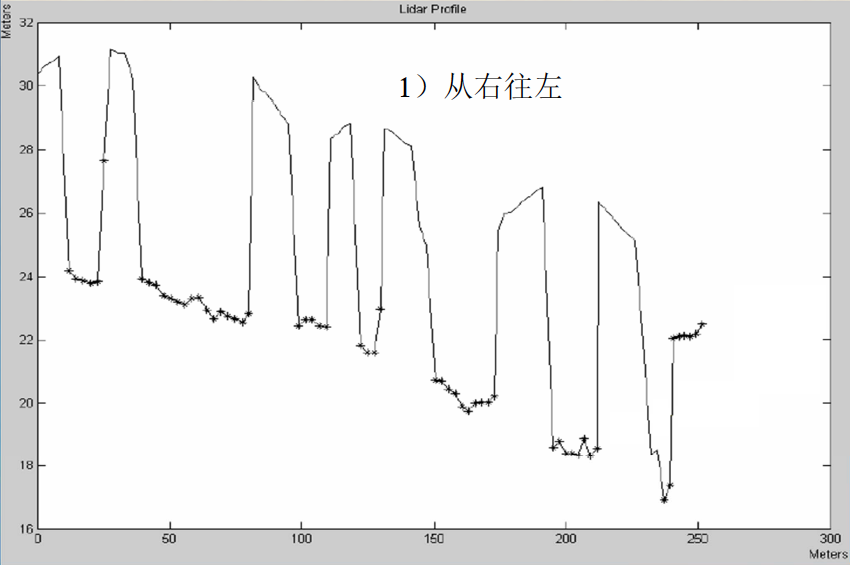
\includegraphics[height=3cm]{figure/Chapter6/一维双向扫描标记法-从右往左}} \quad
			\subfloat[从左往右]{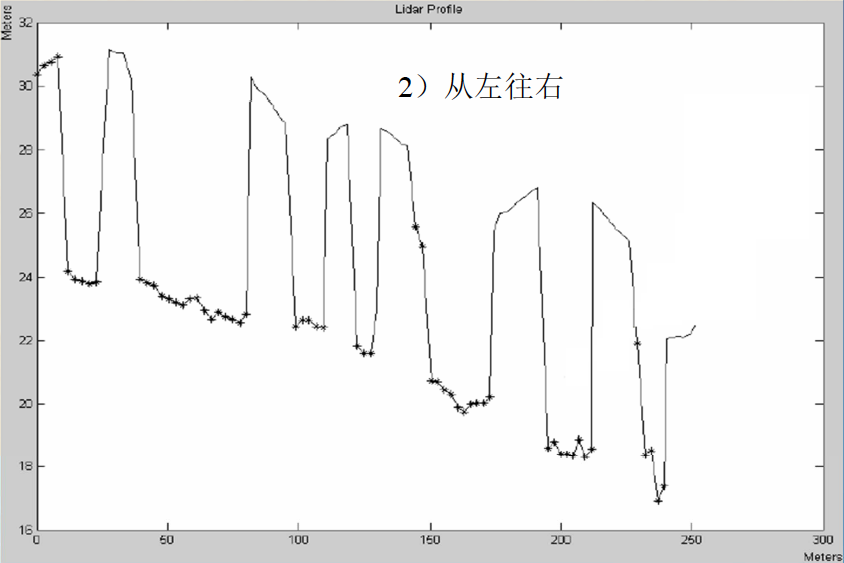
\includegraphics[height=3cm]{figure/Chapter6/一维双向扫描标记法-从左往右}} \\
			\subfloat[取交集]{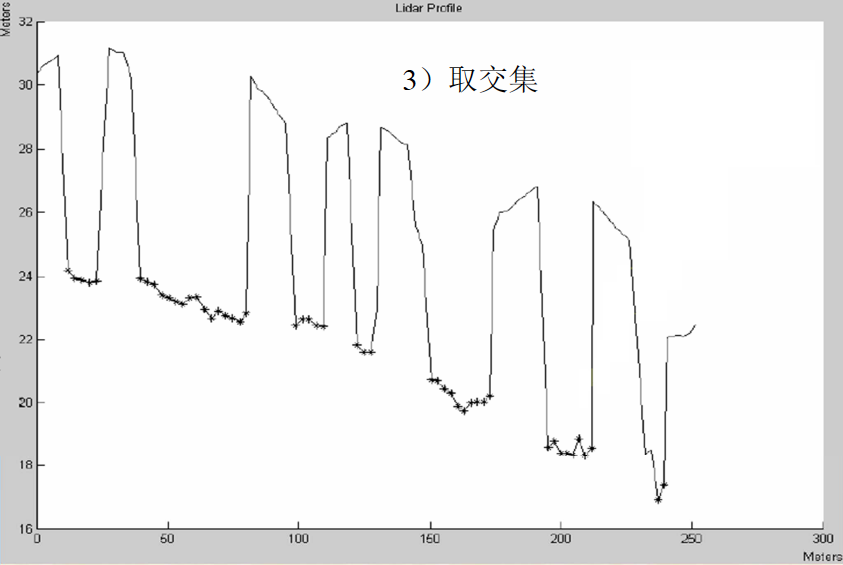
\includegraphics[height=3cm]{figure/Chapter6/一维双向扫描标记法-取交集}} \quad\quad\quad
			\subfloat[线性衰减]{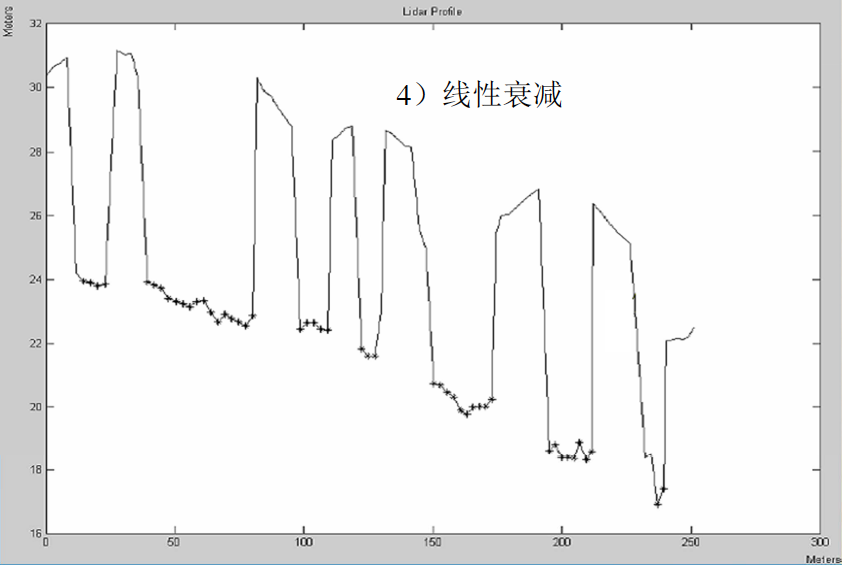
\includegraphics[height=3cm]{figure/Chapter6/一维双向扫描标记法-线性衰减}}
			\caption{一维双向扫描标记法算法步骤}
			\label{fig:一维双向扫描标记法算法步骤}
		\end{figure}
\end{enumerate}

\kaiparagraph{TopScan算法}
\begin{enumerate}
	\item \textbf{步骤过程}:
		\begin{itemize}
			\item 采用比较大的移动窗,在窗中搜索最低点,由每次移动窗中找出的最低点的全体,形成了一个初步的地面模型。
			\item 将所有的点与此模型比较,在每一点上形成高差,凡高差超过某个阈值,被认为是非地面点,将这些点滤除。
			\item 减小窗口,重复第一、二步工作,搜索最低点,形成地面模型,改变阈值,滤除与地面模型高差大的点,重复数次以后得到比较精确的地面点高程数据集合 。
		\end{itemize}
	\item \textbf{窗口和滤波阈值大小的选取}:
		\begin{itemize}
			\item 窗口小,就可能将一些大房屋顶点保留下来;窗口太大 则会将地表面“平滑”,使微小的地形变化部分被滤除。
			\item 阈值太大,会将一些植被点作为地面点保留下来;阈值太小,可能将真实的较小的地形突变点去掉;
			\item 窗口和阈值大小与实际地形地貌密切相关。不同的地域, 如平原、丘陵、山地,应该有不同的参量。
		\end{itemize}
\end{enumerate}

\kaiparagraph{基于多分辨率方向预测的点云滤波算法}
\begin{enumerate}
	\item \textit{线性预测法}:若相邻两点距离比较近,而且二者的高程相差较小,则认为这两点为同一类型点的可能性比较大;
		否则较高点为地物点的可能性比较大。
		当然随着两点之间的距离的加大,较高点为地物点的可能性也随之减小。
			
		假设集合$ S $为原始LiDAR点云,则地面点集合$ S_T $可以表示为
		\begin{equation}
		S_T = \left\lbrace p_i \in S \left| ∀p_j \in S : h_{p_i} - h_{p_j} \leqslant Δh_{\max} \left( d(p_i,p_j) \right) \right. \right\rbrace
		\end{equation}
	\item \textit{方向预测法}:在某一距离范围内,若当前点与所有方向预测值的差值均大于该距离条件下的最大高差限差,则该点为地物点,否则为地面点。
	
		对于原始LIDAR点云属于集合$ S $,方向数据集$ S_{\text{dir}} \in S $,则地物点数据集$ S_O $可以表示为
		\begin{equation}
		S_T = \left\lbrace p_i \in S \left| ∀p_j,p_k \in S_{\text{dir}} : h_{p_i} - h(p_j,p_k) > Δh_{\max} \left( d(p_j,p_k) \right) \right. \right\rbrace
		\end{equation}
		则地面点数据集$ S_T $可以表示为
		\begin{equation}
		S_T = S - S_O
		\end{equation}
	\item \textit{多分辨率方向预测处理}:采用类似影像金字塔的方式,构建不同分辨率的数据集,以分辨率由低到高的次序依次进行平滑处理。邻域方向如图\ref{fig:邻域方向}所示。
		\begin{figure}[htbp]
			\centering
			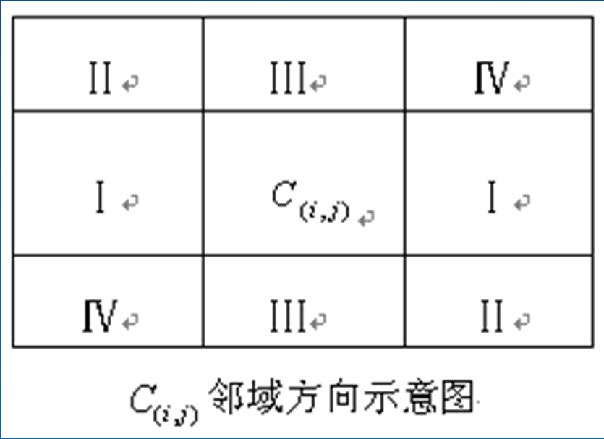
\includegraphics[scale=0.5]{figure/Chapter6/邻域方向}
			\caption{邻域方向}
			\label{fig:邻域方向}
		\end{figure}
\end{enumerate}

\kaiparagraph{移动曲面滤波方法}
\begin{enumerate}
	\item \textbf{算法原理}:激光点云的空间关系反映了地形表面的空间变化,任何一个复杂的空间曲面,其局部面元可利用一个简单的二次曲面拟合
		\begin{equation}
		Z_i = f(X_i,Y_i) = a_0 + a_1 X_i + a_2 Y_i + a_3 X_I^2 + a_4 X_i Y_i + a_5 Y_i^2
		\end{equation}
		当局部面元小到一定程度,甚至可以将该局部面元近似表达成一个平面
		\begin{equation}
		Z_i = f(X_i,Y_i) = a_0 + a_1 X_i + a_2 Y_i
		\end{equation}
	\item \textbf{算法步骤}
		\begin{itemize}
			\item 选择初始地面种子点。选择局部最低的三个点作为种子点(图\ref{fig:移动曲面滤波算法1})。
			\item 进行初始平面拟合(图\ref{fig:移动曲面滤波算法2})。
			\item 基于平面拟合方程判别邻近激光点。当拟合点数达6个时,改用二次曲面方程进行地形拟合(图\ref{fig:移动曲面滤波算法3})。
			\item 基于二次曲面方程进行地面点的迭代判 别,并不断更新地形曲面,完成LiDAR点云的滤波(图\ref{fig:移动曲面滤波算法4})。
		\end{itemize}
		\begin{figure}[htbp]
			\centering
			\subfloat[]{\label{fig:移动曲面滤波算法1}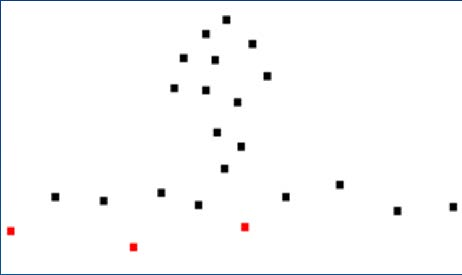
\includegraphics[height=2.2cm]{figure/Chapter6/移动曲面滤波算法1}} \hfill
			\subfloat[]{\label{fig:移动曲面滤波算法2}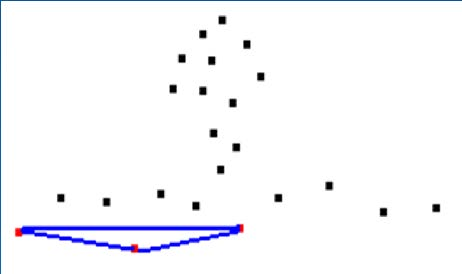
\includegraphics[height=2.2cm]{figure/Chapter6/移动曲面滤波算法2}} \hfill
			\subfloat[]{\label{fig:移动曲面滤波算法3}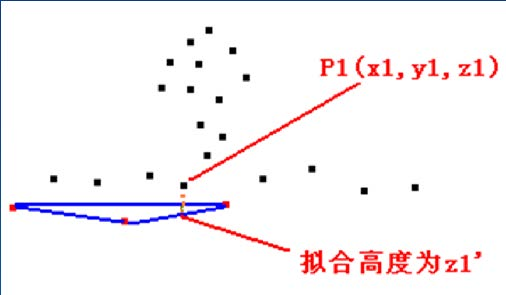
\includegraphics[height=2.2cm]{figure/Chapter6/移动曲面滤波算法3}} \hfill
			\subfloat[]{\label{fig:移动曲面滤波算法4}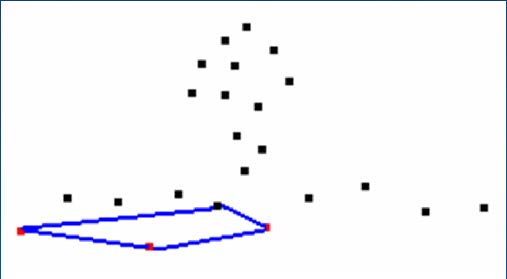
\includegraphics[height=2.2cm]{figure/Chapter6/移动曲面滤波算法4}}
			\caption{移动曲面滤波算法}
			\label{fig:移动曲面滤波算法}
		\end{figure}
	\item \textbf{难点}:该算法的难点在于种子点的选择以及滤波阈值的确定。种子点选择不恰当会使得曲面迭代拟合结果陷入极值,无法得到正确结果;同时滤波阈值需要根据地形起伏自适应地变化,否则难以取得较好的效果。
\end{enumerate}

\kaiparagraph{基于TIN加密的点云滤波方法}
\begin{enumerate}
	\item \textbf{原理}:
		\begin{itemize}
			\item 获取一定的地面种子点组成初始的稀疏不规则三角网;
			\item 对各点进行判断,如果该点到三角面的垂直距离及角度小于设定的阈值,将该点加入地面点集合,实现TIN的不断 加密。
			\item 重新计算不规则三角网,然后再对非地面点集合内的点进行判别。
			\item 如此迭代,直到不再增加新的地面点,或者满足给定条件为止。
		\end{itemize}
	\item \textbf{过程}:
		\begin{itemize}
			\item 采用逐级内插
			\item 逐步迭代,由粗到细的内插方法。
			\item 迭代条件:
				\begin{itemize}
					\item 点与三角形的夹角不能大于一定的限度。
					\item 点与所在三角形的距离不能大于一定的限度。
				\end{itemize}
		\end{itemize}
	\item \textbf{种子点选取思路}:建筑物一般不会覆盖较大的区域(譬如: 80m × 80m)。这个范围内的低点一般是地面点。
	\item \textbf{难点}:
		\begin{itemize}
			\item 需要先将低的噪声点去除,否则会造成没有点可以选入的情况。
			\item 对于低矮植被不容易去除。
			\item 对于陡峭的小山坡也会发生错分的情况。
		\end{itemize}
\end{enumerate}

\paragraph{其他滤波算法}
\begin{enumerate}
	\item \textit{基于数学形态学滤波方法}
	\item \textit{基于TIN的改进滤波方法}
	\item \textit{基于区域增长的点云滤波方法}
\end{enumerate}

\subsection{DEM生成}
\paragraph{DEM内插}地面空白填补滤波之后产生了一些空缺点,如房屋顶点滤除后,应补上所在位置的高程。
\begin{enumerate}
	\item \textit{反距离权重法}(inverse distance weighting)
		\begin{equation}
		f(P) = \left\lbrace \begin{array}{ll}
		\dfrac{\displaystyle{\sum_{i=1}^{n} d_i^{-u} Z_i}}{\displaystyle{\sum_{i=1}^{n} d_i^{-u}}} & ∀P_i,d_i \neq 0 \\
		Z_i & ∃P_i,d_i = 0
		\end{array} \right.
		\end{equation}
	\item \textit{多项式插值法}(interpolating polynomials)
	\item \textit{最近点插值法}(Nearest Neighbor)
	\item \textit{克立格插值法}(Kriging)
\end{enumerate}
不同的插值方法对应不同的插值精度以及插值效率,也适用于不同的插值用途。

\paragraph{DEM模型}
\begin{enumerate}
	\item \textit{规则格网模型}:根据生成DEM的要求,如范围、间距等,由邻近地面点的位置(即$ (X,Y) $坐标)内插规则格网点上的高程才能最终产生 DEM。
	\item \textit{不规则三角网模型}(TIN):直接基于离散地面点构建Delaunay三角网。
	\item \textit{混合模型}:规则格网+TIN。在地形变化小的地方采用低分辨率的规则格网,在地形变化大的地方用TIN。
\end{enumerate}

\subsection{精度分析}

\paragraph{叠加对比分析}如图\ref{fig:叠加对比分析}所示,由激光扫描数据生成的等高线(浅色);由摄影测量方法生成的等高线(深色)。
\begin{figure}[htbp]
	\centering
	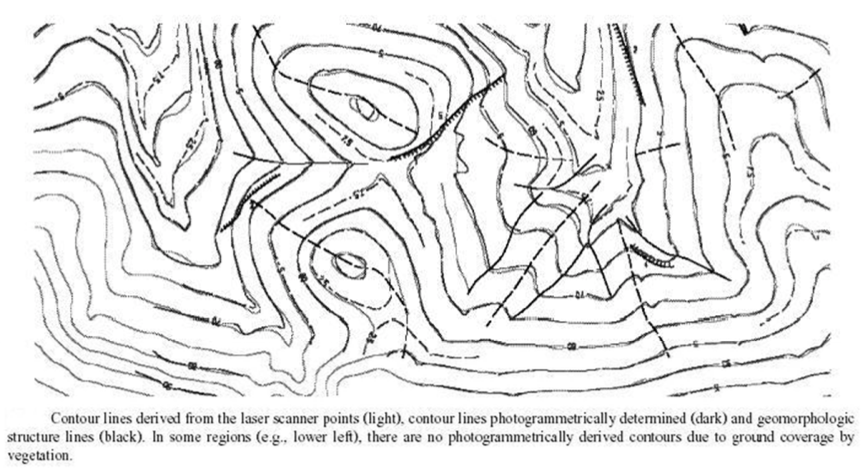
\includegraphics[width=0.8\linewidth]{figure/Chapter6/叠加对比分析}
	\caption{叠加对比分析}
	\label{fig:叠加对比分析}
\end{figure}

\paragraph{抽样统计分析}选择植被较少或没有植被的平坦地区作为检查区域,与差分GPS测量结果进行比较,得到高程残差统计图。如图\ref{fig:抽样统计分析}所示。
\begin{figure}[htbp]
	\centering
	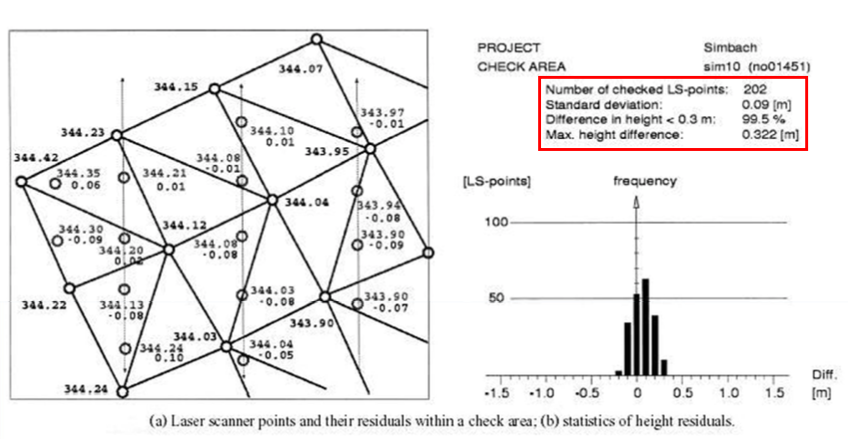
\includegraphics[width=0.8\linewidth]{figure/Chapter6/抽样统计分析}
	\caption{抽样统计分析}
	\label{fig:抽样统计分析}
\end{figure}

\paragraph{LiDAR的优势}
\begin{itemize}
	\item \textbf{费用成本低}:与摄影测量方法比较,所需费用只是其25\%$ \sim $33\%,节省了山区林地地面实测的费用、内业处 理的费用等。
	\item \textbf{限制条件少}:飞行季节、时间、天气的限制较少。
		\begin{itemize}
			\item 冬季也可以进行,既便有雪也无碍;
			\item 白天黑夜都可以工作;
			\item 在阴天,云下飞行扫描同样有较好的结果。
		\end{itemize}
\end{itemize}

\paragraph{建议}
\begin{itemize}
	\item \textbf{时间}:最好在11月到第二年三月间进行;
	\item \textbf{天气}:最好选择无雪、无雨的日子;
	\item \textbf{参量}:飞行和扫描参量根据各种不同需要,在飞行前要认真讨论确定;扫描点的分布要尽可能有规律;对于10 m格网间距高程精度要求数分米的DEM,平均扫描点距不要超过5m。
	\item \textbf{基站}:用于GPS差分处理,对于提高精度非常重要;
	\item \textbf{检测区域}:要选择平地或斜地,植被复盖尽可能少, 量测点密,量测精度要优于1 dm;
	\item \textbf{检测}:95\%的点的精度优于3 dm的情况下才算合格。
\end{itemize}

\section{强度数据处理}
商用LiDAR系统在获取三维位置坐标信息(距离)数
据的同时都可以记录下各激光脚点反射的回波信号的
强度信息。由于强度信息的本质同传统的光学影像是
一样的,大多数学者倾向于采用传统的数字图像处理
的方法来处理。

\subsection{强度数据特点}
\begin{enumerate}
	\item 噪声大
	\item 未定标
	\item 与距离信息同时获取
	\item 与光学影像相似
\end{enumerate}

\subsection{强度数据校正}LiDAR系统记录的强度值与接收回波信号能力成正比,
因为为了使得强度值真实反映目标的反射特性,必须
去掉距离、瞬时角度以及大气和传感器参数等外部影
响。

依据激光雷达方程
\begin{equation}
P_r = \dfrac{\eta_o \rho T_a^2 A_r}{\pi R^2} \cdot \dfrac{A_i}{A_b}P_t
\end{equation}
式中,$ P_r $是激光雷达接收到的激光功率;$ P_t $是光学系统效率;$ \rho $是目标表面反射率,$ T_a $是单程大气透过率,$ A_r $是光学系统有效接触面积,$ R $是目标与激光雷达的距离;$ A_i $是目标被照面积(截面积);$ A_b $是目标处的光斑面积。
经推导得到
\begin{equation}
P_r = \dfrac{P_t D_r^2 \rho}{4R^2} \cos \theta_i \eta_{\text{sys}} \eta _{\text{atm}}
\end{equation}
式中,$ \theta_i $为瞬时角度,$ \eta_{\text{sys}} $为系统发射因子,$ \eta _{\text{atm}} $为大气影响因子。

可借助接收功率与距离、角度等比例关系进行强度校正!

\subsection{强度图像生成处理}
\begin{enumerate}
	\item \textbf{重采样}:将时间序列的数据转换为规则格网数据阵列,每个像素值代表该点对应的回波强度值。
	\item \textbf{去粗差}
	\item \textbf{去噪}:LiDAR强度信息存在着较严重的噪声,噪声中的主要成份为脉冲噪声(椒盐噪声),其概率密度函数(PDF)一般为指数密度分布和伽马密度分布。这种噪声为乘性噪声,与信号相关,本质上是非线性的,难以去除。
		\begin{itemize}
			\item \textit{中值滤波去噪}:常用的非线性滤波方法。中值滤波对脉冲 干扰及椒盐噪声的抑制效果好,在抑制随机噪声的同时,造成边缘模糊成度小。
			
				\textbf{做法}:对一个滑动窗口内的所有像素灰度值排序,用中值作为窗口中心像素输出值的处理。
			\item {\kaishu 针对城区LiDAR强度数据的去噪}
			\item {\kaishu 基于平坦度的LiDAR强度图像去噪}:适用非城区数据处理。
		\end{itemize}
\end{enumerate}

\subsection{应用案例}

结合LiDAR强度和距离信息实现道路的自动提取。

\section{基于LiDAR数据的建筑物提取}

\paragraph{建筑物提取的方法}
\begin{enumerate}
	\item \textbf{基于光学影像的方式}
		\begin{itemize}
			\item 利用单幅影像阴影分析的方法,或直接通过边缘检测获取建筑物边界的方法。
			\item 利用立体像对进行人工判读(模拟及解析测量的成图方式),提取建筑物的方法;
				或利用数字摄影测量工作站进行半自动或全自动的建筑物提取。
		\end{itemize}
	\item \textbf{基于LiDAR点云的方式}:基于LiDAR点云进行建筑物提取即模型重建。
		\begin{itemize}
			\item 建筑物检测(分割)
			\item 建筑物模型生成(重建)
		\end{itemize}
\end{enumerate}

\paragraph{两种提取方法的不同}基于影像的建筑物提取方法与基于LiDAR的建筑物提取方法的不同之处如表\ref{tab:建筑物两种提取方法的不同}所示。
\LTXtable{\linewidth}{table/建筑物两种提取方法的不同}

\subsection{建筑物检测(分割)}

\kaiparagraph{分割}由激光扫描数据建立房屋模型,首先必须将房屋点从点云数据中识别、提取出来。

\paragraph{一般步骤}
\begin{enumerate}
	\item 检测出建筑物激光脚点数据
	\item 确定各建筑物激光脚点所属的建筑物,即建立多对一的映射关系。
\end{enumerate}

\paragraph{现有分割方法}
\begin{itemize}
	\item 在数据密度足够大,地面起伏不大的情况下,可采取局部极值检测方法,并以极值点为中心进行局部直方图分析,得到合理的阙值,实现房屋点的检测。
	\item 采取滤波方法来辅助建筑物的提取。滤波是为了滤除非地面点,可用于房屋点的提取。
	\item 利用激光扫描回波强度数据,作为分析房屋的辅助数据。如对于近红外激光,植被的反射率很高,可以用来区分房屋和植被,但这种反射率数据质量一般较差。
	\item 利用辅助数据源:
		\begin{itemize}
			\item 利用二维GIS信息,即利用已有的图形数据,辅助建筑物数据的提取。但需要注意实际的屋顶面常常比图形数据所显示的面积要大。
			\item 利用影像光谱信息,现有的LiDAR系统在飞行时,会同时载有多光谱和高光谱扫描仪,其影像数据将大大有利于房屋的提取。
		\end{itemize}
\end{itemize}

\paragraph{涉及的处理方法}:高度直方图分析、形态滤波等方法、房屋最低高度阙值、最小屋顶面积等:

\subsection{建筑物模型的生成(重建)}
\paragraph{任务}提取矢量化的建筑物模型。

\paragraph{现状}虽然LiDAR提供了丰富的建筑屋顶面\footnote{屋顶面虽然仅仅是建筑物模型的一个重要部分,但几乎所有的建筑物模型重建研究都集中于屋顶模型的重建。}的信息,但是,由于建筑物结构复杂,自动化程度较高的建筑物模型重建算法、商用软件并没有出现。

\paragraph{建筑物提取的典型方法}
\begin{itemize}
	\item 基于三角网的房屋模型重建方法
	\item 基于不变矩的建筑物提取方法
	\item 自适应迭代的DSM影像分割方法
	\item 基于边界表达的建筑物模型重建方法
	\item 其他:基于特征线的数据驱动方法、Hough变换以及其扩展变换、模型驱动的方法……
\end{itemize}

\kaiparagraph{基于三角网的房屋模型重建方法}
\begin{enumerate}
	\item 分割建筑物点,并构建三角网
	\item 分析三角面元,确定屋顶平面。
		\begin{itemize}
			\item 对每一个小三角平面都可以根据三个定点的坐标,计算出两个坡度参量$ S_x$、$ S_y $和一个距离参量$ d $,因为每一个平面可由下式描述
				\begin{equation}
				Z = S_x X + S_y Y + d
				\end{equation}
			\item 计算出所有小平面的上述参量,形成一个三维参量聚类空间,参量相同的小平面在同一个屋顶面内。
		\end{itemize}
	\item 提取边界线。将各个屋顶面参量求解出来之后,就可以提取边界线和屋脊线。如果有多条脊线,则最长的脊线代表房屋的主方向。
	\item 进行边界优化和拟合
		\begin{enumerate}
			\item 前提条件:
				\begin{itemize}
					\item 边缘线与代表房屋方向的屋脊线平行或垂直;
					\item 主方向的边缘点应当是高程等值点。
				\end{itemize}
			\item 拟合流程:对分割后数据集中处于边缘上的点进行分析:
				\begin{itemize}
					\item 从其中任意一点出发,找到相邻点之后即初步估计出连线的方向,计算出连线的直线方程。
					\item 按该直线方向与房屋走向的关系进行调整,后续点根据它与该直线的距离是否超过某一阂值,决定它是否为该直线方向的边缘点,当超过阂值就是另一条边缘直线的开始点。
					\item 对于初步的搜索结果通过最小二乘拟合进一步优化,使所有边缘点到边缘线的距离平方和最小。
					\item 拟合结果并非边缘线的真正位置,因为边缘线应当将所有边缘点都围在所形成的多边形内,要尽可能使边缘点处于边界内。
					
					可以利用墙面点信息,对边缘线位置作一点调整,墙面点信息是被分割的屋顶点集以外的点,有助于屋顶边缘线的确定,也有助于计算墙面高度。
				\end{itemize}
		\end{enumerate}
\end{enumerate}

\kaiparagraph{利用不变矩提取房屋模型}
\begin{enumerate}
	\item 对于连续函数,矩的定义
		\begin{equation}
		M_{ij} = \int_{x_1}^{x_2}\int_{y_1}^{y_2} x^i y^j f(x,y) \diff x \diff y
		\end{equation}
		LiDAR数据是离散数据,分割之后,按分割的子集分别计算其矩,并以\textbf{高程值作为权重},则矩的定义
		\begin{equation}
		M_{ij} = \sum_{p=p_i}^{p_n} x_p^i y_p^j H_p
		\end{equation}
		$ H_p $为子集$ {p_1,p_2,\cdots,p_n} $中某点的高程。
		
		\textit{不变矩}是各坐标重心化之后,相应于个子集重心的矩。
			\begin{itemize}
				\item \textit{平移不变矩}
				\item \textit{比例不变矩}
				\item \textit{旋转不变矩}
			\end{itemize}
		
		对于灰度化的数据,$ H_p = 1 $,可以得到二值矩$ m_{ij} $定义如下
		\begin{equation}
		M_{ij} = \sum_{p=p_i}^{p_n} x_p^i y_p^j
		\end{equation}
		注意:房屋的参量必须由归一化矩计算得到,即与除以$ m_{00} $进行归一化处理。
	\item 房屋类型的确定:可以通过比较带高程权重的二阶矩与灰度化二阶矩得到,即
		\begin{equation}
		r_q = \dfrac{M_{20}/M_{02}}{m'_{20}/m'_{02}}
		\end{equation}
		\begin{itemize}
			\item 若$ rq=1 $,则屋顶为平面;
			\item 若$ rq>1 $,则屋顶面与房屋主轴平行;
			\item 若$ rq<1 $,则屋顶面与房屋主轴垂直。
		\end{itemize}
	\item 一般步骤
		\begin{itemize}
			\item 房屋点的分割
			\item 确定房屋特征参数与不变矩函数关系式
			\item 计算不变矩,导出房屋特征参数
			\item 利用房屋点及特征参数,计算房屋特征点坐标,并重建房屋模型。
		\end{itemize}
	\item 不变矩的方法常用于计算具有平面或人字形屋顶的房屋的参数。其他屋顶类型的确定需要计算更高阶的矩。更高阶的矩还可以检测屋顶的不对称性。
	\item 不同屋顶类型的处理方法
		\begin{itemize}
			\item 不对称屋顶:首先利用矩确定标
				准的人字形屋顶类型:然后根据实际点云与标准
				模型之间的差异,将其他点(烟囱、天窗、天线
				等)分割出来:最后进一步利用不变矩来分析,
				提取其参数。
			\item 复杂屋顶:将屋顶分割为多个单元,如基元屋
				顶,然后分别提取这些基元屋顶的参数:
			\item 底面形状非矩形的屋顶:不推荐采用高阶不变矩分析的方法来确定其模型。
		\end{itemize}
\end{enumerate}

\kaiparagraph{自适应迭代的DSM影像分割方法}
\begin{enumerate}
	\item \textbf{处理流程}
		\begin{multicols}{2}
			\begin{enumerate}
				\item 城市DSM数据
				\item 中值滤波平滑
				\item 图像阙值分割
				\item 提取建筑物的边界
				\item 建筑物边界眼踪
				\item 去除不闭合的边界
				\item 多边形逼近建筑物
				\item 边界点的分组和拟合方位角
				\item 确定或给定建筑物主方向
				\item 建筑物各边缘线段规格化
				\item 边缘规格化效果评价
				\item 计算建筑物的高度
				\item 建筑物高度填充
				\item 建筑物DSM图像
			\end{enumerate}
		\end{multicols}
	\item \textbf{影像分割}
	\item \textbf{边缘提取}
	\item \textbf{边缘优化处理}
	\item \textbf{高度填充}
\end{enumerate}

\kaiparagraph{基于边界表达的建筑物模型重建方法}
\begin{enumerate}
	\item \textbf{处理流程}
		\begin{itemize}
			\item 建筑物检测:去除地形、树木、其他噪声
			\item 边缘提取
			\item 面特征提取
			\item 特征融合、模型重建
		\end{itemize}
		得到:阶跃边缘、屋脊线、屋顶面片。
	\item \textbf{建筑物检测}
	\item \textbf{建筑物边缘提取}:对于阶跃边缘,计算每个点邻域内$ Z $坐标差异。
	\item \textbf{特征直线检测}:每个点分为9个局部方向,采用\textit{角度分解的方法},每个点投票决定直线,点对直线的贡献,由点到直线的距离产特定。
	\item \textbf{优化内容}:
		\begin{itemize}
			\item 孤立点分类:点到线段的距离决定归属。
			\item 线段合并:将方向想尽、距离相近的线段合并为一条线段。
			\item 线段竞争:最优线段最长,且满足正交关系。
			\item 规则化:边缘垂直、平行处理。
		\end{itemize}
	\item \textbf{屋顶面片检测}:
		\begin{enumerate}
			\item \textbf{思路}
				\begin{itemize}
					\item 屋顶面片检测的常用方法:三维Hough变换。缺点是比较慢,计算量大。
					\item 三角形向量统计方法,由于数据过于密集,三角形小,法向量对噪声十分敏感。
					\item 点法向量统计:用点和其邻域内的点构成的小平面代替三角形计算法向量。
					\begin{figure}[htbp]
						\centering
						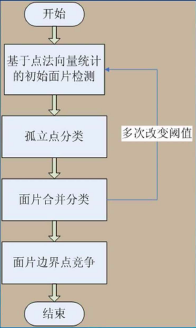
\includegraphics[width=0.3\linewidth]{figure/Chapter6/点法向量统计处理流程}
						\caption{点法向量统计处理流程}
						\label{fig:点法向量统计处理流程}
					\end{figure}
				\end{itemize}
			\item \textbf{面片检测顺序}
				\begin{itemize}
					\item 安高程直方图进行区域增长
					\item 按面片法向进行面片竞争和屋脊线检测。
				\end{itemize}
			\item \textbf{屋顶面的分裂与合并}:消除虚假边缘,得到完整的屋顶面。
				\begin{itemize}
					\item \textit{分裂}:充分利用已经检测到的建筑物边缘作为初始条件和约束,寻找两个不同类型的区域之间最合适的边界。
					\item \textit{合并}:将那些属于建筑物的同质区域合并起来,则可以形成闭合的建筑物边界多边形,这就是普通测图需要完成的一项重要工作一一建筑物轮廓线生成。
					
					\textbf{合并的优先级}
						\begin{itemize}
							\item 大块优先合并
							\item 合并朝着使对象几何特性更加规则的方向进行
							\item 注意边界坚固性对合并的影响,如图\ref{fig:边界坚固性}。
								\begin{figure}[htbp]
									\centering
									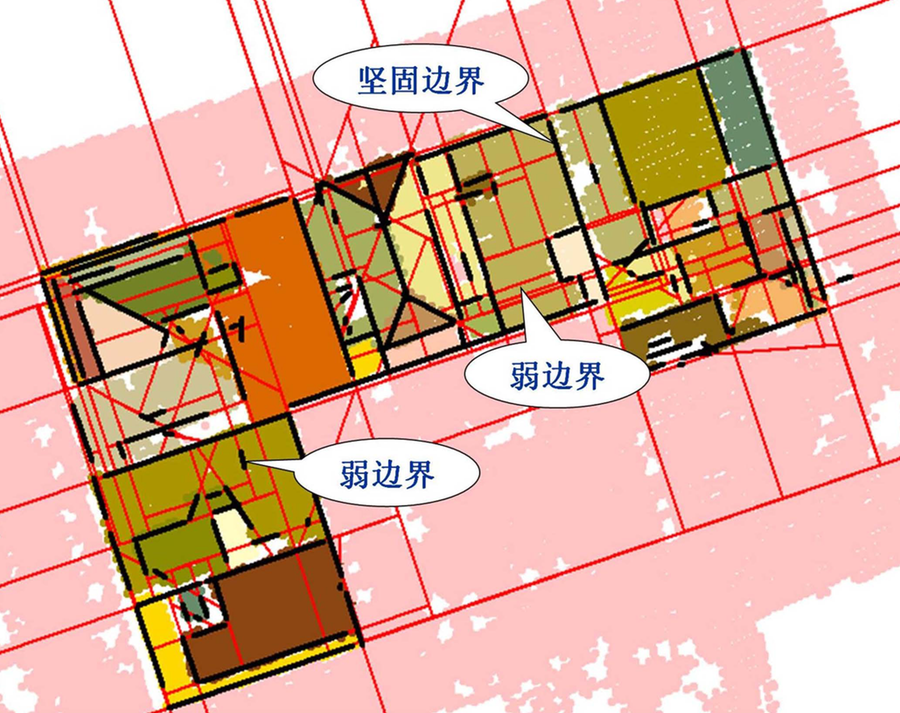
\includegraphics[width=0.5\linewidth]{figure/Chapter6/边界坚固性}
									\caption{边界坚固性}
									\label{fig:边界坚固性}
								\end{figure}
						\end{itemize}
				\end{itemize}
		\end{enumerate}
\end{enumerate}

\subsection{三维重建质量检查}

\paragraph{城市三维重建误差来源}如表\ref{tab:城市三维重建误差来源}所示。
\begin{table}[htbp]
	\centering
	\caption{城市三维重建误差来源}
	\label{tab:城市三维重建误差来源}
	\begin{tabular}{|>{\bfseries}c|>{\kaishu}c|l|}
		\hline
		\multicolumn{2}{|c|}{\thead{数据处理过程}} & \thead{误差来源} \\\hline
		\multirow{5}{*}{数据源} & 航片资料 & 几何变形、灰度变形、参数精度 \\\cline{2-3}
								& 待更新数据 & 数据精度、准确性、现势性 \\\cline{2-3}
								& DEM数据 & 数据精细程度、精度 \\\cline{2-3}
								& 纹理数据 & 纹理映射误差 \\\cline{2-3}
								& 属性数据 & 禹性逻辑错误、完备性 \\\hline
		\multirow{4}{*}{生产过程} & 早期数据纠正 & 自己准精度、定向精度 \\\cline{2-3}
								& 数据采集 & 仪器、人员、定向精度、采集方式 \\\cline{2-3}
								& 数据建模 & 数据格式转换 \\\cline{2-3}
								& 数据编辑 & 编辑原则、编辑方法、操作人员 \\\hline
	\end{tabular}
\end{table}

\paragraph{三维重建质量检查}从三维重建的角度来看,三维模型检查主要包括几何模型检查和拓扑结构检查。
\begin{enumerate}
	\item \textbf{几何模型的检查}:将建立的三维模型跟立体像对中的立
		体模型进行比照,检查三维模型几何结构的正确性,并
		确定精度超限需要重新量测的地物。实践中可以按点、
		线、面与体的不同层面来检查其模型结构的正确性。对
		应不同的层面其检查方式和检查内容也有区别:
		\begin{itemize}
			\item \textit{点检查}:主要是检查平面位置是否正确、同高的点是否同高。
			\item \textit{线检查}:主要是检查地物边缘垂直、平行条件是否满
				足。如房屋边缘大部分表现为垂直与平行结构,但在
				实际量测过程中一般难以满足。当前普遍采用的方法
				是对不满足垂直与平行结构的部分,使用格网功能进
				行编辑改正。
			\item \textit{面检查}:主要是检查面结构是否合理,共面误差是否满足给定的限度。
			\item \textit{体检查}:模型高度是否正确,组合是否完整,几何结构是否合理。
		\end{itemize}
	\item \textbf{拓扑结构检查}:遍历三维模型并与影像对中的立体影像对照,检查三维模型的拓扑结构是否正确,其主要内容包括:
		\begin{itemize}
			\item \textit{目视检查}:根据立体模型检查所建立的三维模型在视觉上是否与立体影像在主要结构特征上一致。
			\item \textit{冗余面检查}:检查是否存在破坏面完整性的冗余面。
			\item \textit{外拓扑检查}:复杂房屋及其附属设置间的拓扑关系。
		\end{itemize}
\end{enumerate}

\paragraph{质量控制策略}
\begin{enumerate}
	\item \textbf{生产过程的质量约束}
	\item \textbf{误差补偿}
		\begin{itemize}
			\item \textit{自动补偿}:通过数学方法对系统误差和随机误差的不确定因素进行模拟估计从而进行补偿。
			\item \textit{人机交互补偿}:对不能用数据方法模拟的随机误差,利用误差检测算法检测超限模型采用人机交互进行补偿的方法。
		\end{itemize}
\end{enumerate}

\section{基于LiDAR的道路提取*}

\section{分类、变化检测及波形处理}

\subsection{LiDAR点云分类}

\paragraph{地物目标分类}基于不同地物目标在遥感数据中表现不
同的特性,采取合适的判别方法(函数),将
其划分为不同的类别,制作成专题图,供用户
使用。

\textbf{分类算法的通用性}:设计分类算法时,首先要确
定各种对象的定义,这些定义要尽可能地一般化
(通用)——能较好地适应大多数的地貌。

\paragraph{目标对象的定义}如图\ref{fig:LiDAR数据中的对象}所示。
\begin{itemize}
	\item \textit{地貌}:裸露地面及地面上对象构成的场景
	\item \textit{裸露地面}:分段连续、光滑的曲面
	\item \textit{地面上对象}:自然对象、人造对象
	\item \textit{分离对象}
	\item \textit{附着对象}:桥梁等
	\item \textit{局外对象}:系统误差、远离地貌的对象
\end{itemize}

\begin{figure}[htbp]
	\centering
	\subfloat[地貌]{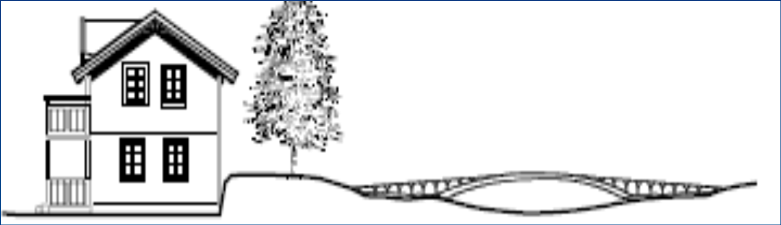
\includegraphics[height=2cm]{figure/Chapter6/地貌}} \hspace{4em}
	\subfloat[裸露地面]{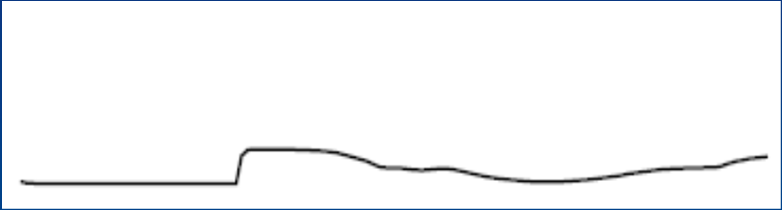
\includegraphics[height=2cm]{figure/Chapter6/裸露地面}} \\
	\subfloat[地物对象]{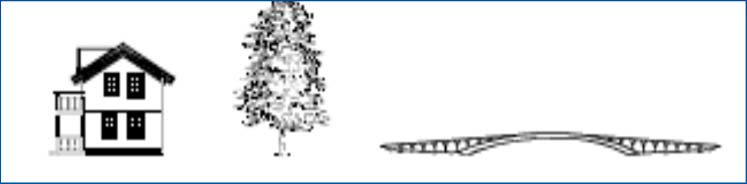
\includegraphics[height=2cm]{figure/Chapter6/地物对象}} \hfill
	\subfloat[附着对象]{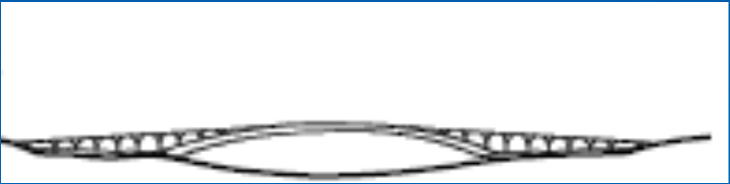
\includegraphics[height=2cm]{figure/Chapter6/附着对象}} \\
	\subfloat[分离对象]{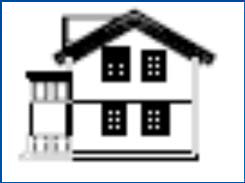
\includegraphics[height=2cm]{figure/Chapter6/分离对象}} \hspace{4em}
	\subfloat[局外对象]{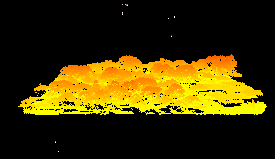
\includegraphics[height=2cm]{figure/Chapter6/局外对象}}
	\caption{LiDAR数据中的对象}
	\label{fig:LiDAR数据中的对象}
\end{figure}

\paragraph{地物点数据的几何特点}
\begin{enumerate}
	\item \textbf{建筑物的几何特点}:沿一条扫描线分析
		\begin{itemize}
			\item 建筑物顶面多是平面,在一条扫描线中表现为一条直线,数据的二阶导数应当为零。
			\item 屋脊线或屋顶面交线处,二阶导数不为零。
		\end{itemize}
		对于一般建筑物,沿扫描线的几何模型可以表示为:若某点处$ \dfrac{∂^2 Z}{∂x^2} = 0 $,则该点为线段中点;若$ \dfrac{∂^2 Z}{∂x^2} ≠ 0 $,则该点为直线间断点。其中,$ x $是沿扫描线方向的坐标,$ Z $表示高程。
	\item \textbf{植被数据的几何模型}:$ \dfrac{∂^2 Z}{∂x^2} ≠ 0 $且二阶导数值连续随机分布。
	\item \textbf{电力线}:电力线和植被都具有多重回波特点,因此在分析时还需借助回波强度信息,因为它们的回波强度不同。
	
		此外,要保证分析结果的正确性,得到初步结果后,还需要根据电力线彼此平行,及每一根电力线上各点形成线性结构的特点,采取Hough变换分析方法,以准确地提取电力线。
\end{enumerate}

\paragraph{LiDAR数据分类依据}
\textbf{LiDAR的数据源有}:高程数据、强度数据、同步采集的数码影像。利用这些信号针对不同地物制定约束规则,逐步将地物区分开来。
\begin{itemize}
	\item 高程突变信息;
	\item 地物几何特征;
	\item 强度信息;
	\item 多次回波信息(波形信息);
	\item 影像光谱信息。
\end{itemize}

\paragraph{LiDAR分类规则}
\begin{enumerate}
	\item \textbf{局外对象}:明显高于或低于周围的环境
	\item \textbf{裸露地面}:
		\begin{enumerate}
			\item 基于连续、光滑的裸露地面的定义假设:
				\begin{itemize}
					\item 在水平邻域内,裸露地面点的高度限定在一定的范围内
					\item 裸露地面点的梯度、曲率限定在一定的范围内
					\item 裸露地面在局部和全局上都是相对平坦的
				\end{itemize}
			\item 基于分段连续、光滑的裸露地面定义的假设:裸露地面点及其k近邻所表达的局部曲面片是相对平坦的。
		\end{enumerate}
	\item \textbf{植被}:
		\begin{itemize}
			\item 表面较粗糙;
			\item 多次回波间存在高度差,在同 平面位置$ (X,Y) $处由多重回波得到几个高度值。
		\end{itemize}
	\item \textbf{建筑物}:
		\begin{itemize}
			\item 垂直突出于裸露地面之上
			\item 占据一片连续的区域
			\item 除了部分建筑物边缘,其它部分均不反射多重回波。根据这个特性有可能区分植被和建筑物。
		\end{itemize}
	\item \textbf{电力线}:电力线一般有两次回波
		\begin{itemize}
			\item 激光照射电力线后,被电力线反射形成回波。
			\item 一部分激光绕过电力线照射到地面,形成二次回波。
		\end{itemize}
\end{enumerate}

\paragraph{地物的强度信息}虽然激光脉冲的
反射强度受不同
因素的影响,包
括回波总数,目
标的材质以及脉
冲的入射角等。
但有研究表明强
度数据可以辅助
地表目标的分类。

\paragraph{影像特征辅助点云分类}
\begin{itemize}
	\item 尽管LiDAR数据能够直接获得目标的空间三维点云,对于区分垂直方向特征明显的地物(例如房屋、高大植被)具有极大的优势,但是却难以区分物体表面的材质和结构差异。
	\item 光学遥感影像提供了丰富的、水平连续的光谱信息,但获取的主要是地物表面的信息,有些地物(如建筑物
	和水泥地)的异物同谱和同物异谱现象突出,仅靠光学影像信息分类,困难较大。
	\item 针对不同传感器的优点和局限性,将多源数据融
	合以弥补单个数据源的局限性是一个非常重要的研究
	方向。
\end{itemize}

\subsection{变化检测}

\kaiparagraph{变化检测}
\begin{itemize}
	\item \textit{广义变化检测}:根据不同时间的多次观测来确
		定某个物体的状态变化或确定某现象的变化发展过程。
	\item \textit{遥感影像变化检测}:利用多时相获取的覆盖同
		一地表区域的遥感影像及其它辅助数据来确定和分析地表变化。
\end{itemize}

\paragraph{地物几何变化的表现形式}如图\ref{fig:地物几何变化的表现形式}所示。
\begin{itemize}
	\item 出现或消失
	\item 大小或形状发生变化
	\item 空间位置发生变化
	\item 多种变化形式的组合
\end{itemize}

\begin{figure}
	\centering
	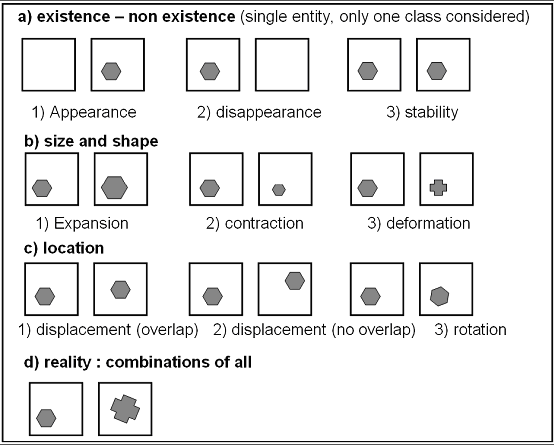
\includegraphics[width=0.7\linewidth]{figure/Chapter6/地物几何变化的表现形式}
	\caption{地物几何变化的表现形式}
	\label{fig:地物几何变化的表现形式}
\end{figure}

\paragraph{变化监测的主要内容}
\begin{itemize}
	\item 检测和判断是否发生了变化;
	\item 标定变化发生的区域;
	\item 确定变化的性质(对于多时相数据,也称变化的轨迹);
	\item 评定变化检测结果的精度;
	\item 评估变化的时间和空间分布模式。
\end{itemize}

\paragraph{变化监测方法分类}
\begin{enumerate}
	\item \textbf{基于影像的变化检测}:根据遥感信息灰度值的变化而进行检测。
		\begin{itemize}
			\item \textit{分类后比较}:先对不同时相的原始影像分别进行分类解译,然后比较
				各时相分类结果图来发现变化,同时确定变化类型。其过程如图\ref{fig:分类后比较}所示。
				\begin{figure}[htbp]
					\centering
					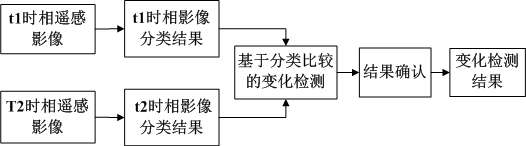
\includegraphics[width=0.5\linewidth]{figure/Chapter6/分类后比较}
					\caption{分类后比较}
					\label{fig:分类后比较}
				\end{figure}
			\item \textit{直接比较}:直接比较同一位置上不同时相的像元特征值来检测变化,
				通常是先采用数学变换的方式生成不同时相间的差异影像,
				再对差异影像进行阈值化处理,从中提取变化区域。其过程如所示。
				\begin{figure}[htbp]
					\centering
					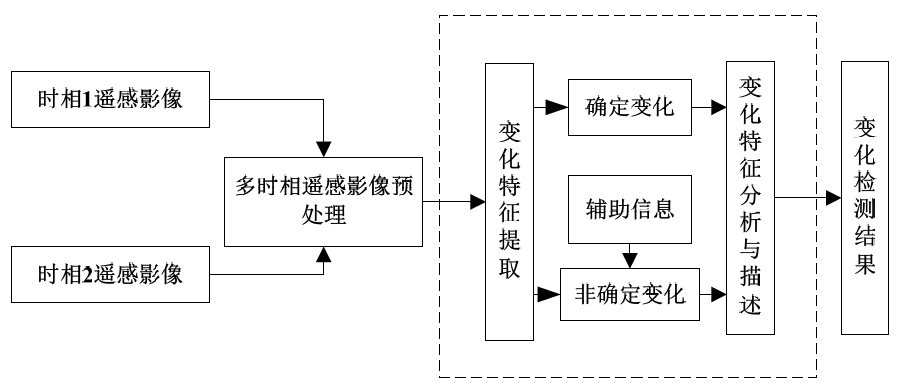
\includegraphics[width=0.5\linewidth]{figure/Chapter6/直接比较}
					\caption{直接比较}
					\label{fig:直接比较}
				\end{figure}
		\end{itemize}
	\item \textbf{基于高程的变化检测}:宫鹏曾使用数字摄影测量工作站和加利福尼亚州丘陵区及佛罗里达州滩涂区的多时相航空摄影立体像对, 构建数字表面模型,用以测量河沟侵蚀、河道窄化和 深切以及海岸带滩涂地带盐沙地的移动,精度达到1 m以内。
		这种方法的自动化程度很低,主要是人工对于正射影像和数字高程模型产品的研究和比较。
		\begin{figure}[htbp]
			\centering
			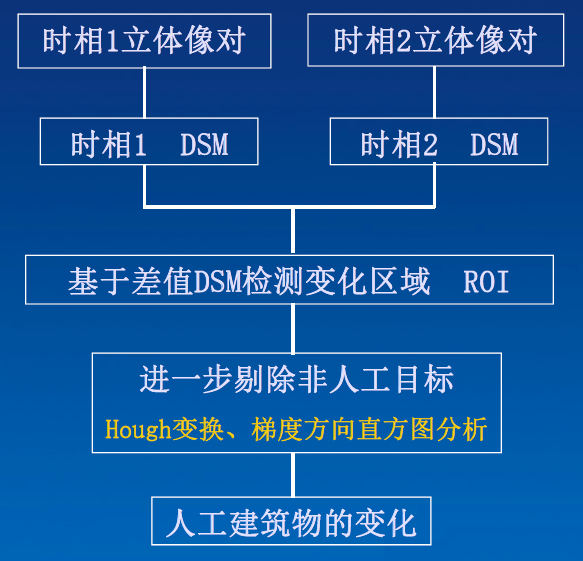
\includegraphics[width=0.5\linewidth]{figure/Chapter6/基于高程的建筑物变化检测流程}
			\caption{基于高程的建筑物变化检测流程}
			\label{fig:基于高程的建筑物变化检测流程}
		\end{figure}
\end{enumerate}

\paragraph{基于变化检测实现城市空间信息数据库的更新}
\begin{itemize}
	\item 采用人工判读航片方式,精度高,但周期长、代价大。
	\item 基于影像灰度的变化检测方法,结果可靠性有待提高,且难以检测高程方面的变化;
	\item 基于立体像对进行高程变化检测的方法:虽然技术上已十分成熟,但对于城市地区,房屋密度比较大,影像匹配常常失败。
	\item 适宜采用LiDAR数据的变化监测
\end{itemize}

\subsection{数码影像处理}

\paragraph{LiDAR系统的数码影像}主要目的是为LiDAR点云数据提供辅助的光谱影像信息,帮助获得纹理和分类的信息;存在着光谱影像与激光点云的配准问题;LiDAR系统中的数码相片经过解算后,得到与点云 数据一致的坐标。一般将影像结合点云(DSM)数据,制作\textit{真正射影像}(True Ortho Image)。

\kaiparagraph{真正射影像}:真正射影像和正射影像的差别,体现在建筑物的纠正
上,由于DEM没有建筑物的高度信息,在纠正时只能按照地面的高度进行纠正,造成了一定的偏差,采用
具有建筑物信息的DSM就不存在这个问题,能够得到正确的投影位置。

\paragraph{真正射影像纠正原理}如图\ref{fig:真正射影像纠正原理}所示。

\begin{figure}[htbp]
	\centering
	\subfloat[透视投影问题]{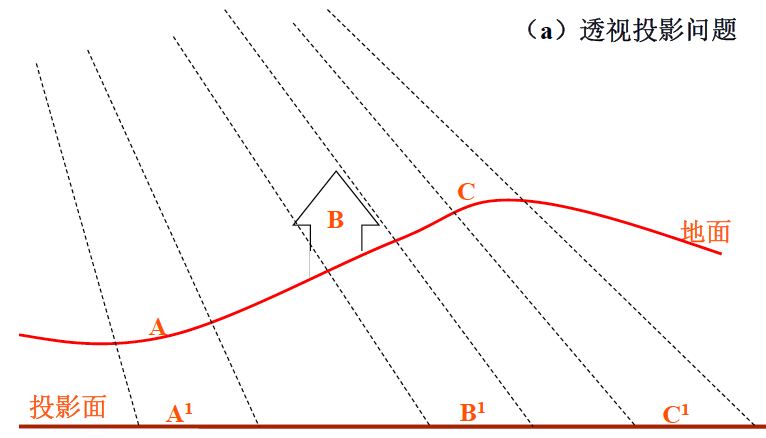
\includegraphics[height=3cm]{figure/Chapter6/透视投影问题}}
	\subfloat[使用DEM纠正的正射影像]{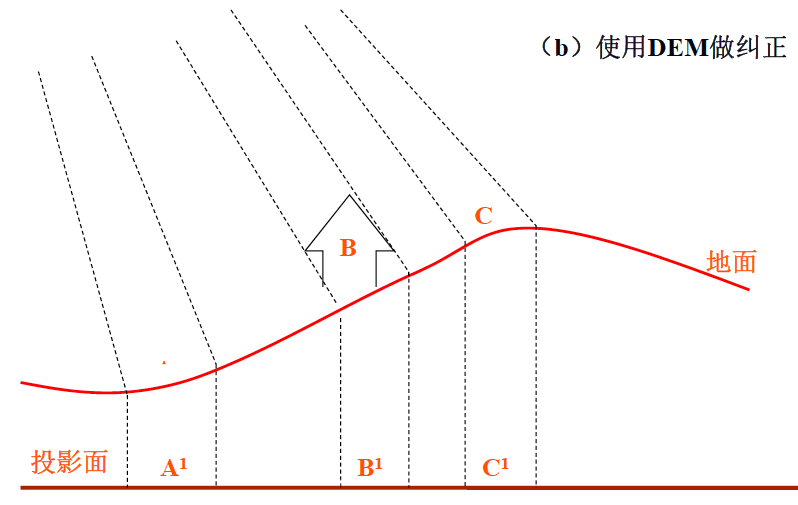
\includegraphics[height=3cm]{figure/Chapter6/使用DEM纠正的正射影像}}
	\subfloat[使用DSM纠正的真正射影像]{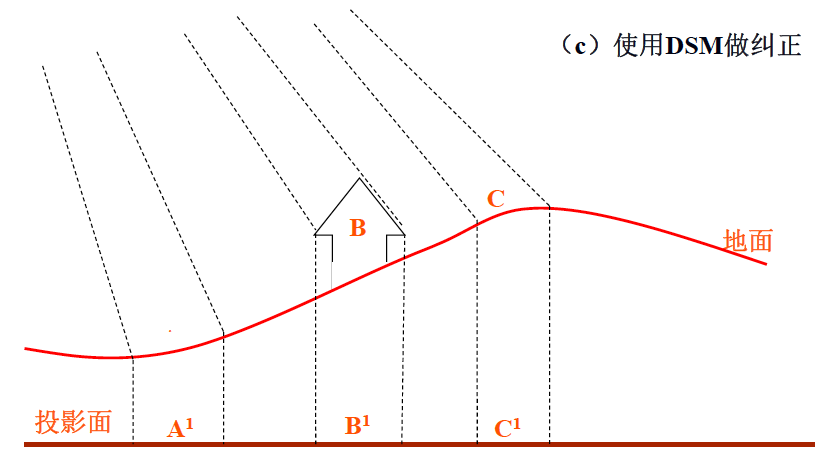
\includegraphics[height=3cm]{figure/Chapter6/使用DSM纠正的真正射影像}}	
	\caption{真正射影像纠正原理}
	\label{fig:真正射影像纠正原理}
\end{figure}

\paragraph{数字正射纠正的两种方式}如图\ref{fig:数字正射纠正的两种方式}所示。
\begin{itemize}
	\item 反解法(间接法):从纠正后影像的像点出发,反求其在原始影像上像点坐标的方法。
	\item 正解法(直接法):从纠正前原始影像的像点出发,计算纠正后该像点的坐标的方法。
\end{itemize}

\begin{figure}[htbp]
	\centering
	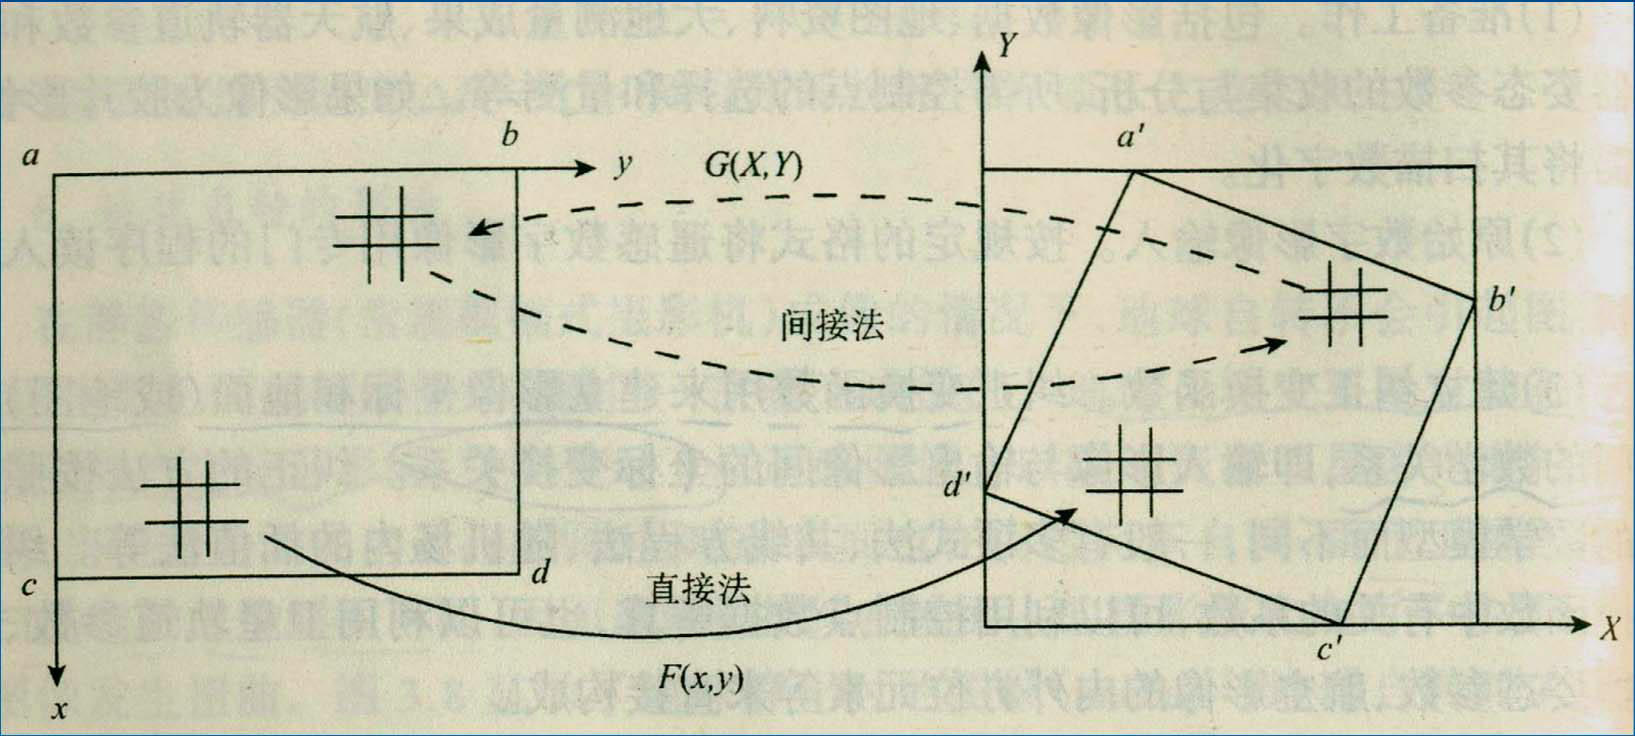
\includegraphics[width=0.7\linewidth]{figure/Chapter6/数字正射纠正的两种方式}
	\caption{数字正射纠正的两种方式}
	\label{fig:数字正射纠正的两种方式}
\end{figure}

\paragraph{存在的问题}
\begin{itemize}
	\item DSM精度不高,导致影像质量下降。
	\item 有的地区缺少纹理。
	\item LiDAR点云有空缺。
	\item 点云与影像配准的问题。
\end{itemize}

\paragraph{解决方案}
\begin{enumerate}
	\item \textbf{房屋边缘的问题}:建筑物边缘不清晰。
	
		\textbf{原因}:点云密度不足。
		
		\textbf{解决方法}:DEM+DBM+影像。地形起伏纠正采用DEM,建筑物纠正采用DBM。以LiDAR原始点云滤波过后得到的DEM和数字建
			筑物模型DBM为基础,建立TIN结构的DSM
	\item \textbf{纹理缺失}
		\begin{itemize}
			\item 遮蔽检测
			\item 纹理选择
			\item 纹理修复
		\end{itemize}
\end{enumerate}

\section{波形处理技术}

\paragraph{激光信号的特点}
\begin{itemize}
	\item 激光束及其回波信号的能量都是连续的。
	\item 多次回波,是将回波能量进行探测和量化之后得到的。 
	\item 探测和量化方法不当会引起误差。
\end{itemize}

\paragraph{激光回波数据处理}如图\ref{fig:激光回波数据处理方法}所示。
\begin{itemize}
	\item 多次回波数据处理
	\item 全波形数据处理
\end{itemize}

\begin{figure}[htbp]
	\centering
	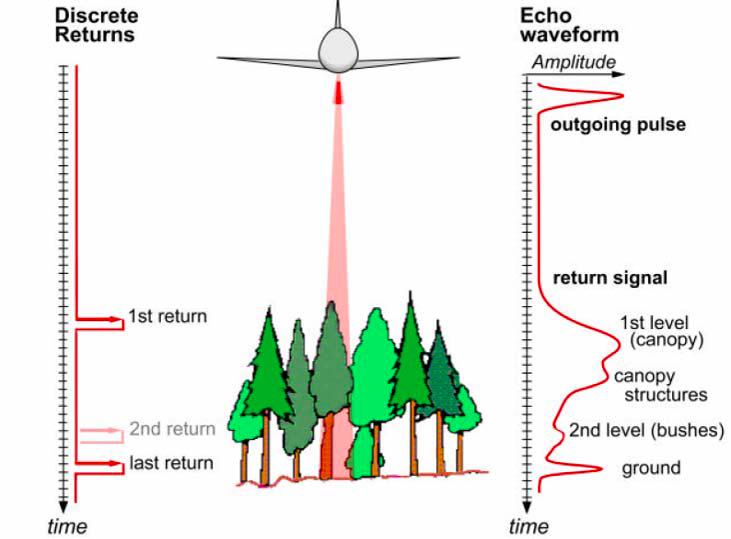
\includegraphics[width=0.5\linewidth]{figure/Chapter6/激光回波数据处理方法}
	\caption{激光回波数据处理方法}
	\label{fig:激光回波数据处理方法}
\end{figure}

\paragraph{多次回波数据处理}
通常将首次和末次回波进行相减,这样可以得
到具有多次回波信息的地物的信息。

\paragraph{全波形数据处理}
对于激光信号还有一种不同的量化方法,即将发
射信号和回波信号均以很小的采样间隔进行采样并加以记录,而不是仅仅提供若干次离散的回波信号,
这就是所谓的\textit{波形数据}(full-waveform)。
\begin{enumerate}
	\item \textbf{特点}:激光回波信号是由发射脉冲和激光光斑内的地物、
		地面共同决定的。地形的起伏以及地表的粗糙度
		对波形都有一定的展宽效应。如图\ref{fig:展宽效应}所示。
		\begin{figure}[htbp]
			\centering
			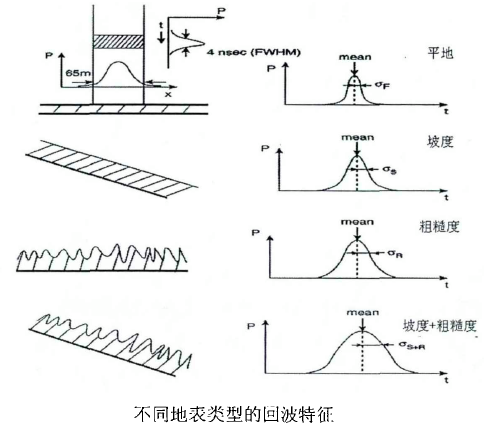
\includegraphics[width=0.5\linewidth]{figure/Chapter6/展宽效应}
			\caption{展宽效应}
			\label{fig:展宽效应}
		\end{figure}
	\item \textbf{分类}
		\begin{itemize}
			\item \textit{星载大脚印全波形数据}
			\item \textit{机载小脚印全波形数据}
				\begin{itemize}
					\item 可以得到更多数量的激光脚点。
					\item 可以得到更多次的回波数据。
					\item 用户更了解数据采集的实际情况,可以采取更合 适的方法进行解算,得到更高精度的点位坐标。
					\item 如果使用波形分解方法,能够得到每次地面目标 反射的波形,进而得到振幅(强度信息)、回波宽度、回波位置和反射系数等参数。
				\end{itemize}
		\end{itemize}
\end{enumerate}

\paragraph{波形数据分解}
全波形数据需要进行分解,以确定反射点(激光脚点)的位置。
\begin{enumerate}
	\item {\bfseries\kaishu 脉冲探测方法}:将波形按时间进行分析和判别,直接探测回波数据的极大值点作为目标的位置。
		\begin{enumerate}
			\item \textit{阈值探测法}:将整个波形数据看作整体,采用一定的阈值(时间、面积的百分比、上升沿等)进行判断,
				得到不同时刻的点坐标,作为不同目标地物的位置。
			\item \textit{均方差判别法}(ASDF):认为LiDAR的反射波是一个混合波,该混合波由一系列的单个波组成的。
				这些单个波是发射波(参考波)经过时间延迟的变化得到的,这些变化包括振幅、宽度等参数。
				ASDF方法使用某种标准,采用局部最优的判断方法,得到极大值点位信息
				\begin{equation}
				R_{\text{ASDF}}(\tau) = \dfrac{1}{N} = \sum_{k=1}^{n} \left( x_1 (kT) + x_2 (kT + \tau) \right)^2
				\end{equation}
		\end{enumerate}
	\item {\bfseries\kaishu 波形分解方法}:通过波形分解的方法能够得到振幅(强度信息)、
		回波宽度、回波位置和反射系数等参数,波形数据的应用研究大多是基于这些参数的进行的。
		
		小光斑波形数据的分解大多基于\textit{高斯分解原理}的方法。这种方法认为,LiDAR的回波波形是由若干个单 一高斯函数的线性叠加而成的,这些高斯函数的振幅、峰值位置、波形宽度、峰值与峰值之间的间距等都是后续波形分析中的重要参数。
			\begin{enumerate}
				\item {\kaishu EM算法}:将LiDAR的全波形数据视为一个高斯混合模型,
					其主要目的是找出一组高斯参数使其符合原波形的期望值,
					并以最大似然法(Maximum Likelihood)来计算这些期望值的估值。
					\begin{itemize}
						\item \textbf{原理}:
							假设波形是由一系列简单的高斯分布组成,则混合分布的数学表示式为
							\begin{equation}
							f(x) = \sum_{j=1}^{k}p_j \times f_j(x),\quad f_j(x) \in N(\mu_j,\sigma_j^2)
							\end{equation}
							式中,$ k $是高斯函数的数量(波峰数量);$ f_j(x) $是每个单一高斯分布的概率密度函数;$ p_j $是权,表示该分布在混合分布中占的比重,满足$ 0 < p_j < 1 $且$ \displaystyle{\sum_{j=1}^{k}p_j = 1} $;$ \mu_j $是均值,$ \sigma_j $是标准差。
							
							EM算法计算高斯混合模型的参数最大似然估计值为
							\begin{align}
							Q_{ij} & = \dfrac{p_j f_j(x)_i}{\displaystyle{\sum_{j=1}^{k} p_j f_j(x_i)}} \\
							   p_j & = \dfrac{\displaystyle{\sum_{i=1}^{s} N_i Q_{ij}}}{\displaystyle{\sum_{i=1}^{s} N_i}} \\
							   \mu_j & = \ddfrac{\sum_{i=1}^{s} N_i Q_{ij} i}{p_j \sum_{i=1}^{s} N_i} \\
							 \sigma_i & = \sqrt{\ddfrac{\sum_{i=1}^{s} N_i Q_{ij} (i - \mu_j)^2}{p_j \sum_{i=1}^{s} N_i}}
							\end{align}
							$ s $是整个波形采样的个数,$ N_i $是每个采用$ i $的强度值,$ p_j $是权值。
						\item \textbf{步骤}:在进行EM算法之前必须先估计高斯混合模型内的高斯函数的个数以及各函数的高斯参数的初值。
							\begin{itemize}
								\item 确定参数初值$ P_j $、$ \mu_j $、$ \sigma_j $、$ k $代入上述各式重新计算参数。
								\item 重复上述步骤,知道满足迭代终止条件。
							\end{itemize}
					\end{itemize}
				\item {\kaishu LM分解方法}:最小二乘法同样假设全波形是由多个单一波线性
					组合而成,且每个单一波满足高斯分布函数。必
					须事先给出单一波的个数,一般先统计波形信息,
					以波峰的个数决定单一波的个数。
					
					建立高斯形态的非线性数学公式
					\begin{equation}
					w(t) = \sum_{j=1}^{k} A_j \exp \left[ - \dfrac{(t-\mu_j)^2}{2\sigma_j^2} \right]
					\end{equation}
					式中,$ k $为波峰数,$ A_j $为振幅,$ t $为时间,$ \mu_j $与$ \sigma_j $为高斯函数的平均值与标准差。
					
					对上式组成观测方程组,待求参数为$ A_j $、$ \mu_j $、$ \sigma_j $。假设假设各单一波为等权且不相关,以最小二乘法求解,其参数解如下式
					\begin{equation}
					x = (B^{\symrm{T}}PB)^{-1}B^{\symrm{T}Pl}
					\end{equation}
					$ x $为改正数,$ B $为系数矩阵,$ P $为权矩阵,$ L $为观测向量。
			\end{enumerate}
\end{enumerate}

